
%(BEGIN_QUESTION)
% Copyright 2010, Tony R. Kuphaldt, released under the Creative Commons Attribution License (v 1.0)
% This means you may do almost anything with this work of mine, so long as you give me proper credit

When sulfur-containing fuels are burned, one of the reaction products is sulfur dioxide (SO$_{2}$), which is an atmospheric pollutant.  Fortunately, SO$_{2}$ is relatively easy to ``scrub'' out of hot flue gases by spraying water down on the rising gases and then chemically treating (regenerating) the resulting solution:

$$\includegraphics[width=15.5cm]{i03042x01.eps}$$

The reaction product formed between water and SO$_{2}$ gas has a strongly corrosive pH value.  Identify what this reaction product is, based on your knowledge of chemistry, and then explain what happens in the ``regenerating'' process to remove this product so that the water may be returned to the scrubber for re-use.

\vskip 10pt

Suppose the sulfur content of the fuel being burned were to increase.  How would this change in fuel chemistry affect the various pH measurements shown in the scrubber process, all other conditions being unchanged?  

\vskip 10pt

Specifically, what kind of ``neutralizing reagent'' must be added to the solution to regenerate it, and what kind of ``waste'' product is generated as a result?

\vskip 20pt \vbox{\hrule \hbox{\strut \vrule{} {\bf Suggestions for Socratic discussion} \vrule} \hrule}

\begin{itemize}
\item{} Rank the four pH transmitters in order of their expected pH measurements, from lowest (acid) to highest (alkaline).
\item{} Explain what would happen to the four pH transmitters' indications if the regenerator process shut down, merely passing water through it without neutralizing pH.
\item{} Explain what would happen to the process if the control valve failed in the shut position.
\item{} Explain what would happen to the process if the control valve failed in the full-open position.
\item{} Identify what kind of pollution hazard is posed by SO$_{2}$ stack emissions.
\item{} Identify suitable flowmeter technologies for the flow measurement points shown in this diagram.
\item{} Would it be worthwhile to install a pH analyzer on the flue gas line?  Explain why or why not.
\end{itemize}

\underbar{file i03042}
%(END_QUESTION)





%(BEGIN_ANSWER)

The reaction product of water and SO$_{2}$ gas is H$_{2}$SO$_{3}$ -- {\it sulfurous acid}.

%(END_ANSWER)





%(BEGIN_NOTES)

Since the reaction product is acidic, it must be treated with added caustic in the regenerating process.  The resulting salt (some ionic ``sulfite'' compound containing SO$_{3}$) may be removed by precipitation or filtration.

%INDEX% Process: flue gas "wet" scrubber 

%(END_NOTES)


